\PH{I have to say I don't remember all these control regions well and
  the fact that the definitions are somewhere else really confuses
  me. I really think it would be good to put a reminder or table or
  discussion in each section.}
Bremsstrahlung photons emitted by beam halo muons in the ECAL volume generate a physical EM shower in the ECAL crystals~\cite{Halo2015}. 
Large deposits energy are rare, but the rate of beam halo penetration
during the 2016 run was substantial. \PH{deposits energy => energy deposits}
The characteristic features of a shower caused by a halo particle include coincident hits in the barrel muon system and a ``trail'' of low-energy clusters in ECAL along the particle trajectory. 
The beam halo MET filter described in Section~\ref{sec:pf_met} exploits the former, while the \emip\ variable described in Section~\ref{sec:pf_photons} captures the latter.

\begin{figure}[htbp]
  \centering
  \resizebox{\textwidth}{!}{
    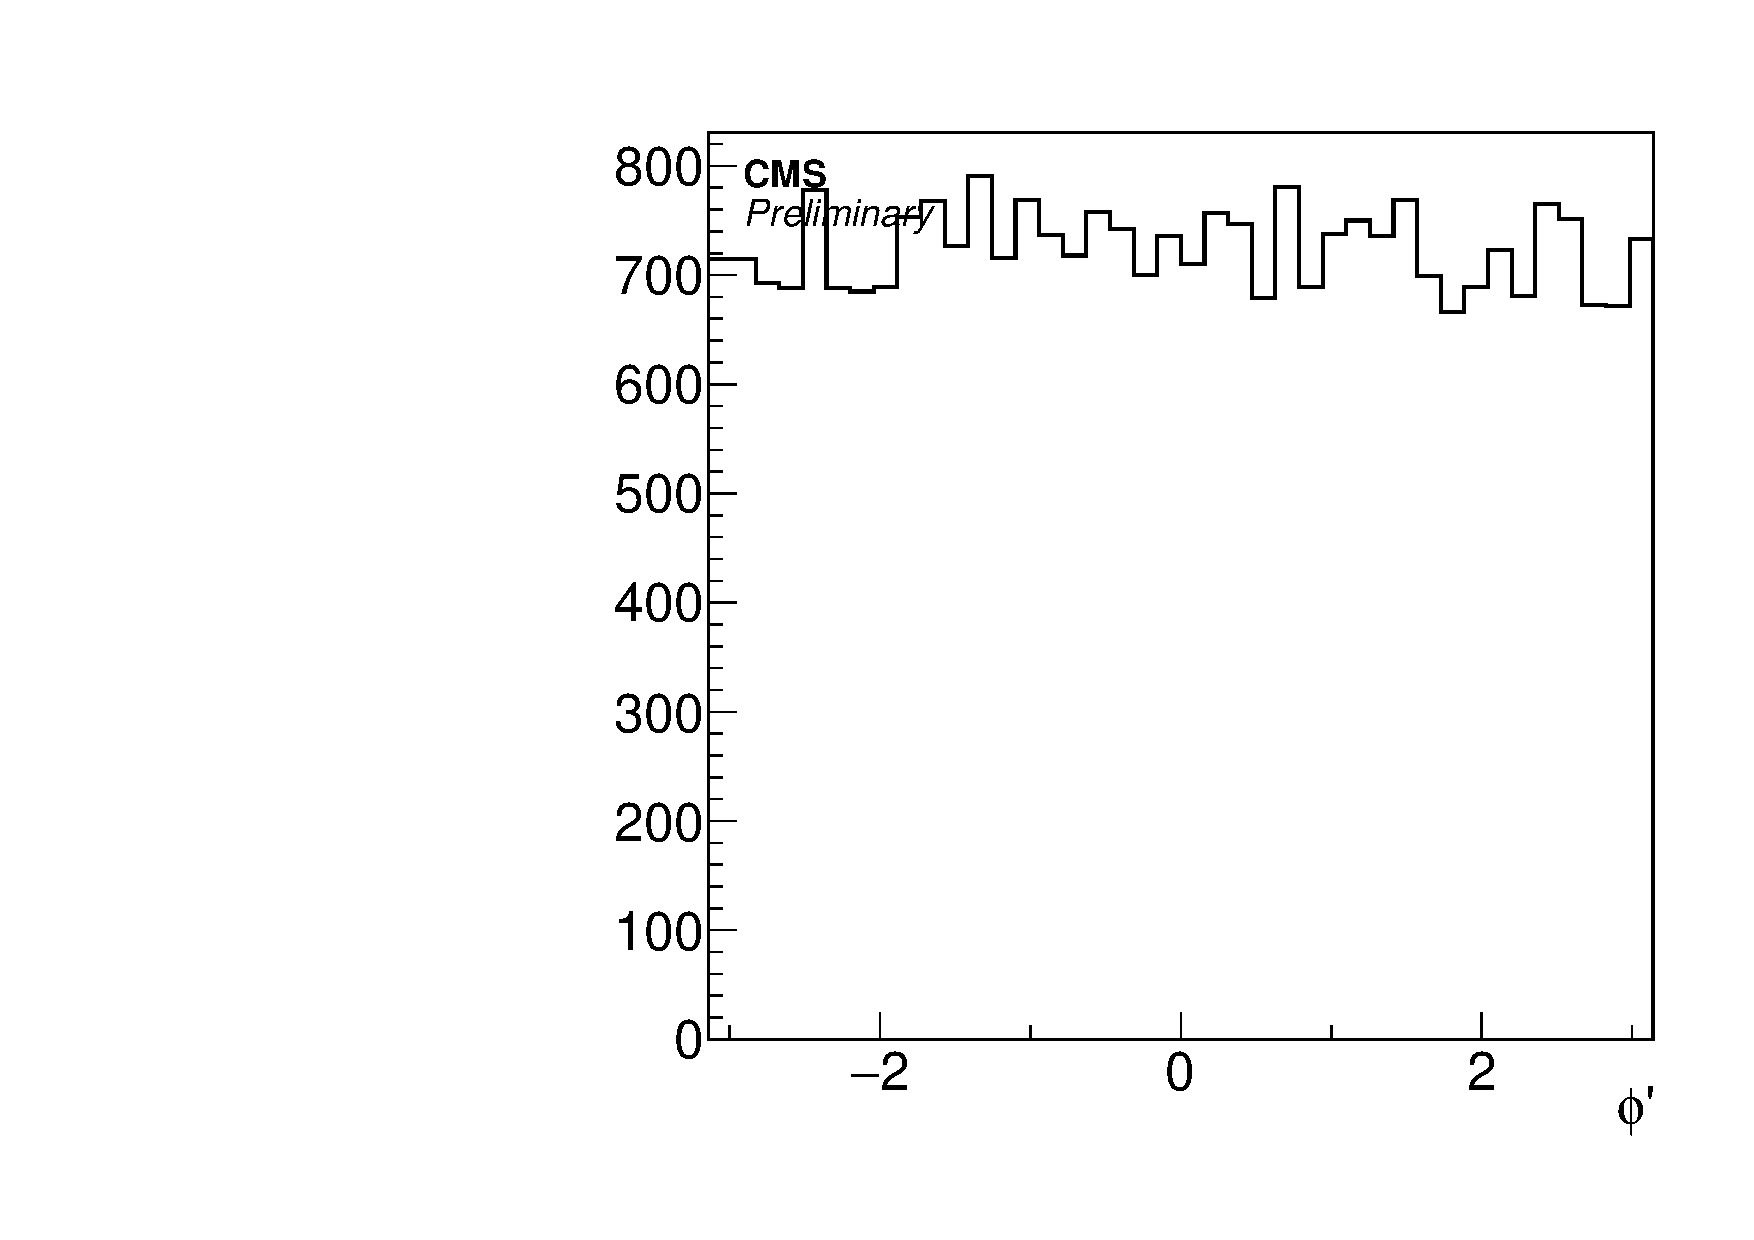
\includegraphics[]{Reconstruction/Figures/halo/bkgphi.pdf}
    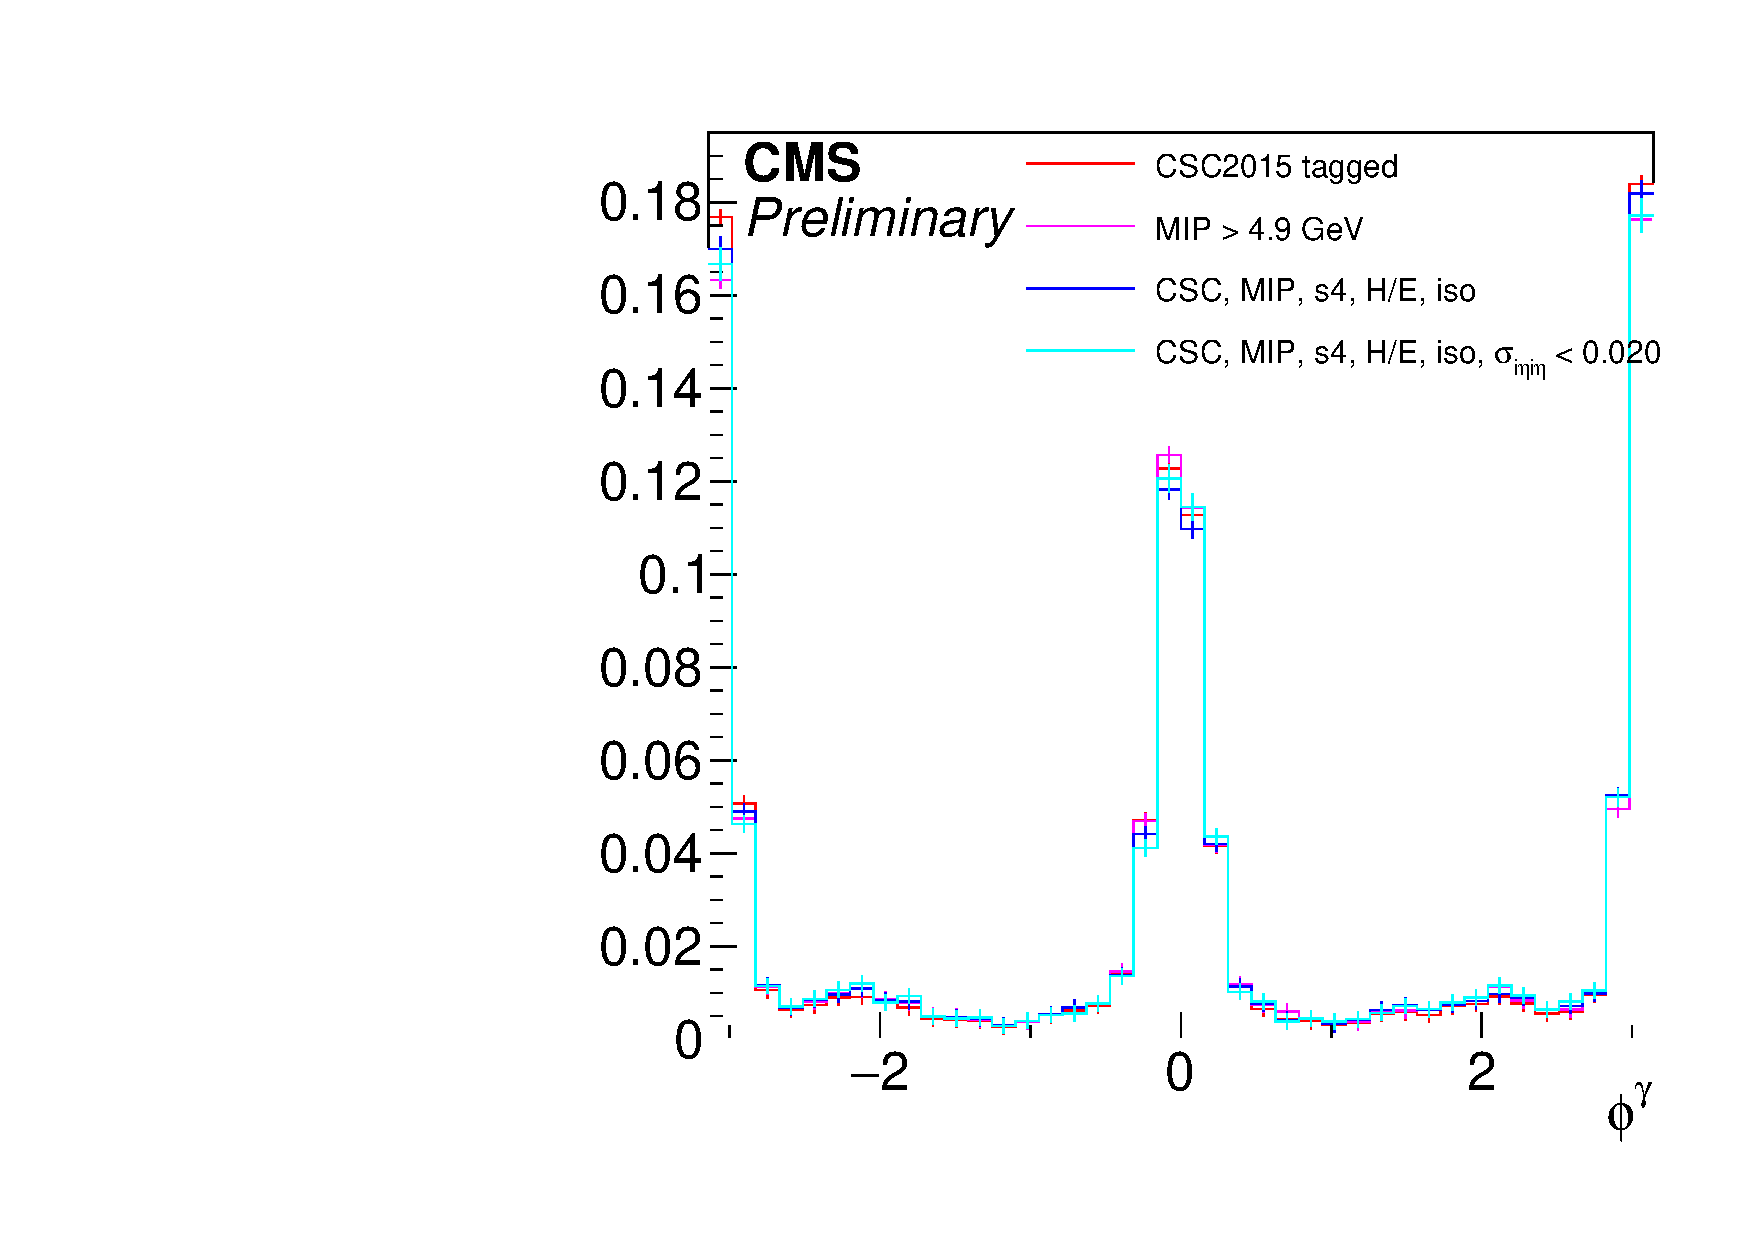
\includegraphics[]{Reconstruction/Figures/halo/halophi.pdf}
  }
  \caption{
    Left: The \phig\ distribution from \zinvg\ MC simulation. \qquad \qquad
    Right: The \phig\ distribution of the halo-like showers, tagged in multiple ways. 
    Histograms are normalized to unity.
    The cyan histogram is the \phig\ distribution after applying photon identification selections except for the shower shape. 
    It can be seen that the \phig\ distribution is highly stable against the listed identification selections.
  }
  \label{fig:halophi}
\end{figure}

Because beam halo particles are produced through complex LHC machine effects, the observed distribution of the halo showers is not
symmetric in the azimuthal angle in the detector coordinates.
The right side of Figure~\ref{fig:halophi} is a \phig\ distribution of the halo showers obtained from the SinglePhoton dataset, requiring $\met > 140\GeV$. 
Halo showers are defined as those that fail the MIP-tagging and in the
event tagged by the CSC beam halo tagger. \PH{in the event tagged by
  ==> tagged by?}
On the other hand, reconstructed showers from all other sources are symmetric in \phig\, as shown on the left side of Figure~\ref{fig:halophi}. 

\begin{figure}[htbp]
  \centering
  \resizebox{\textwidth}{!}{
    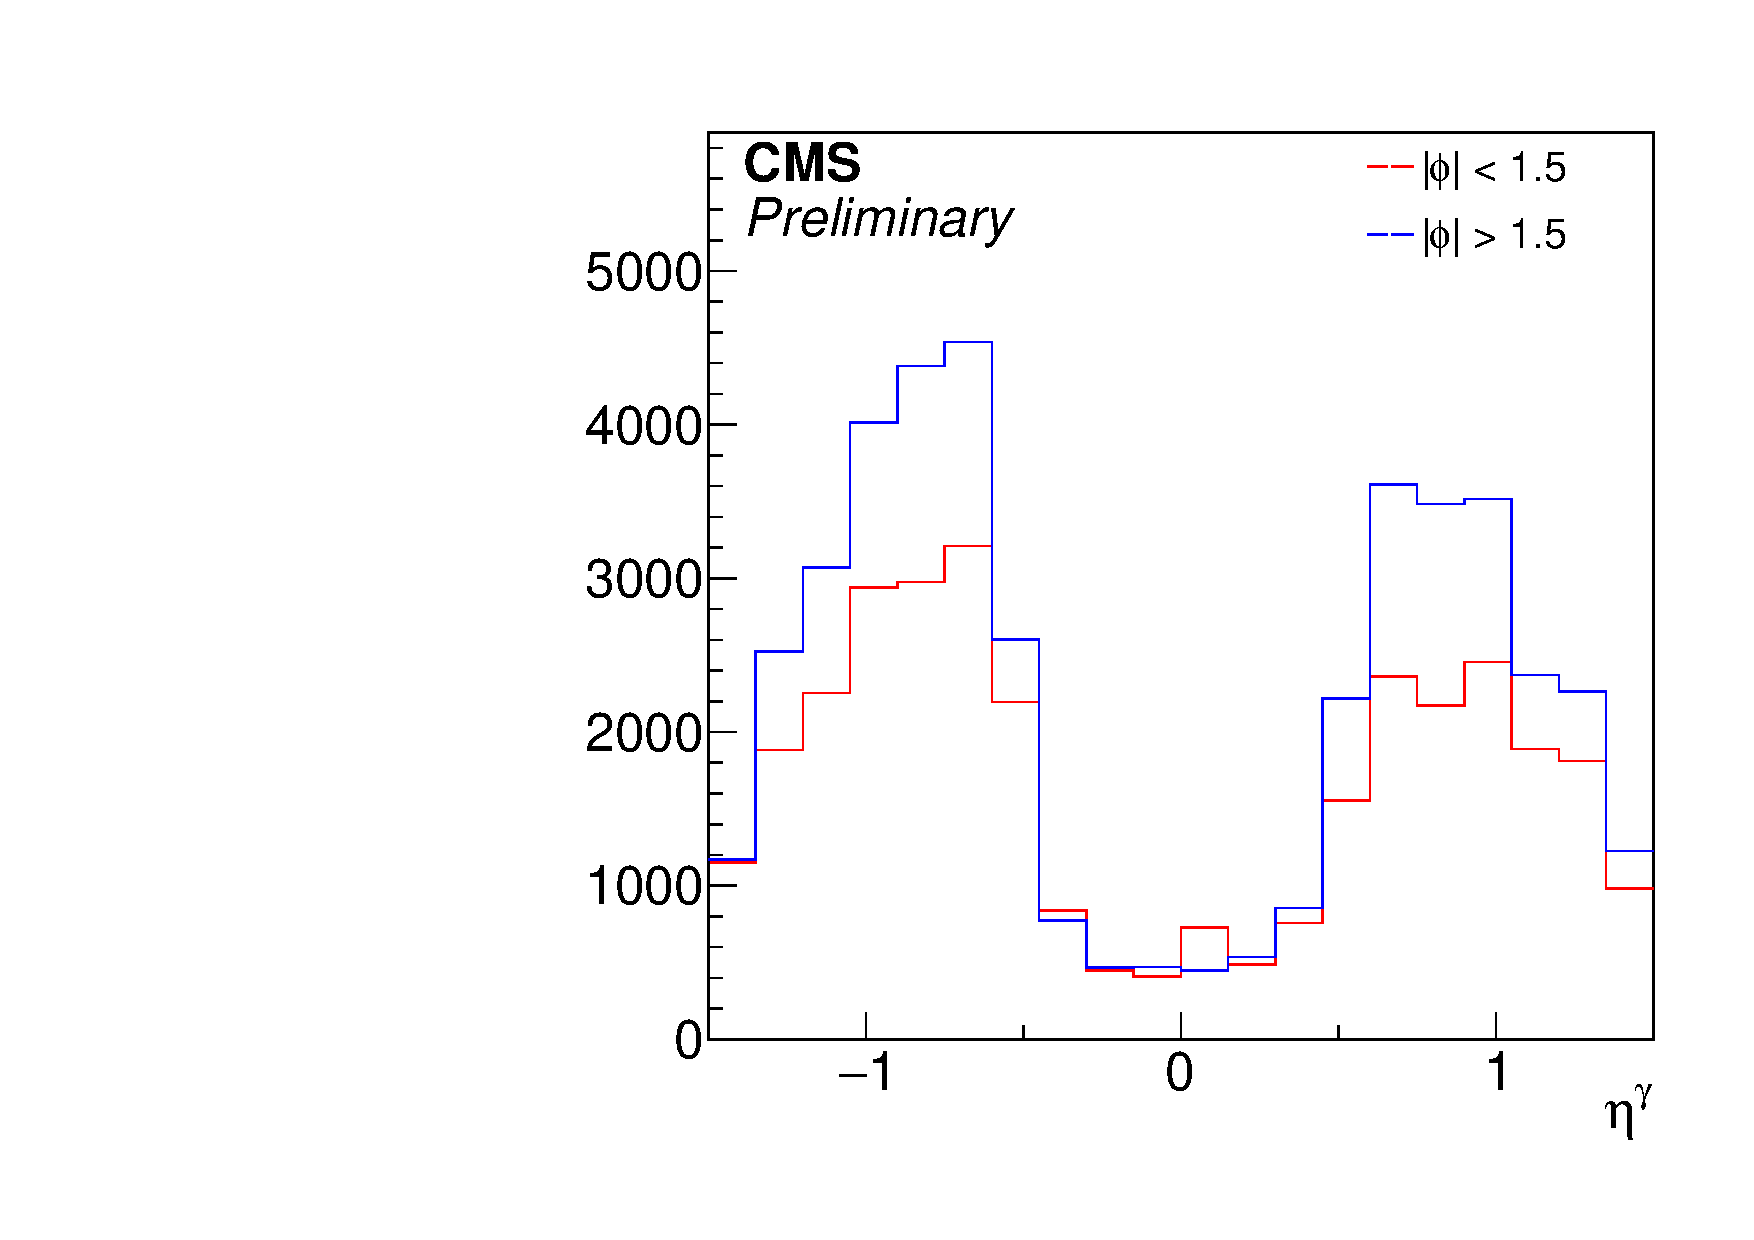
\includegraphics[]{Reconstruction/Figures/halo/halo_eta.pdf}
    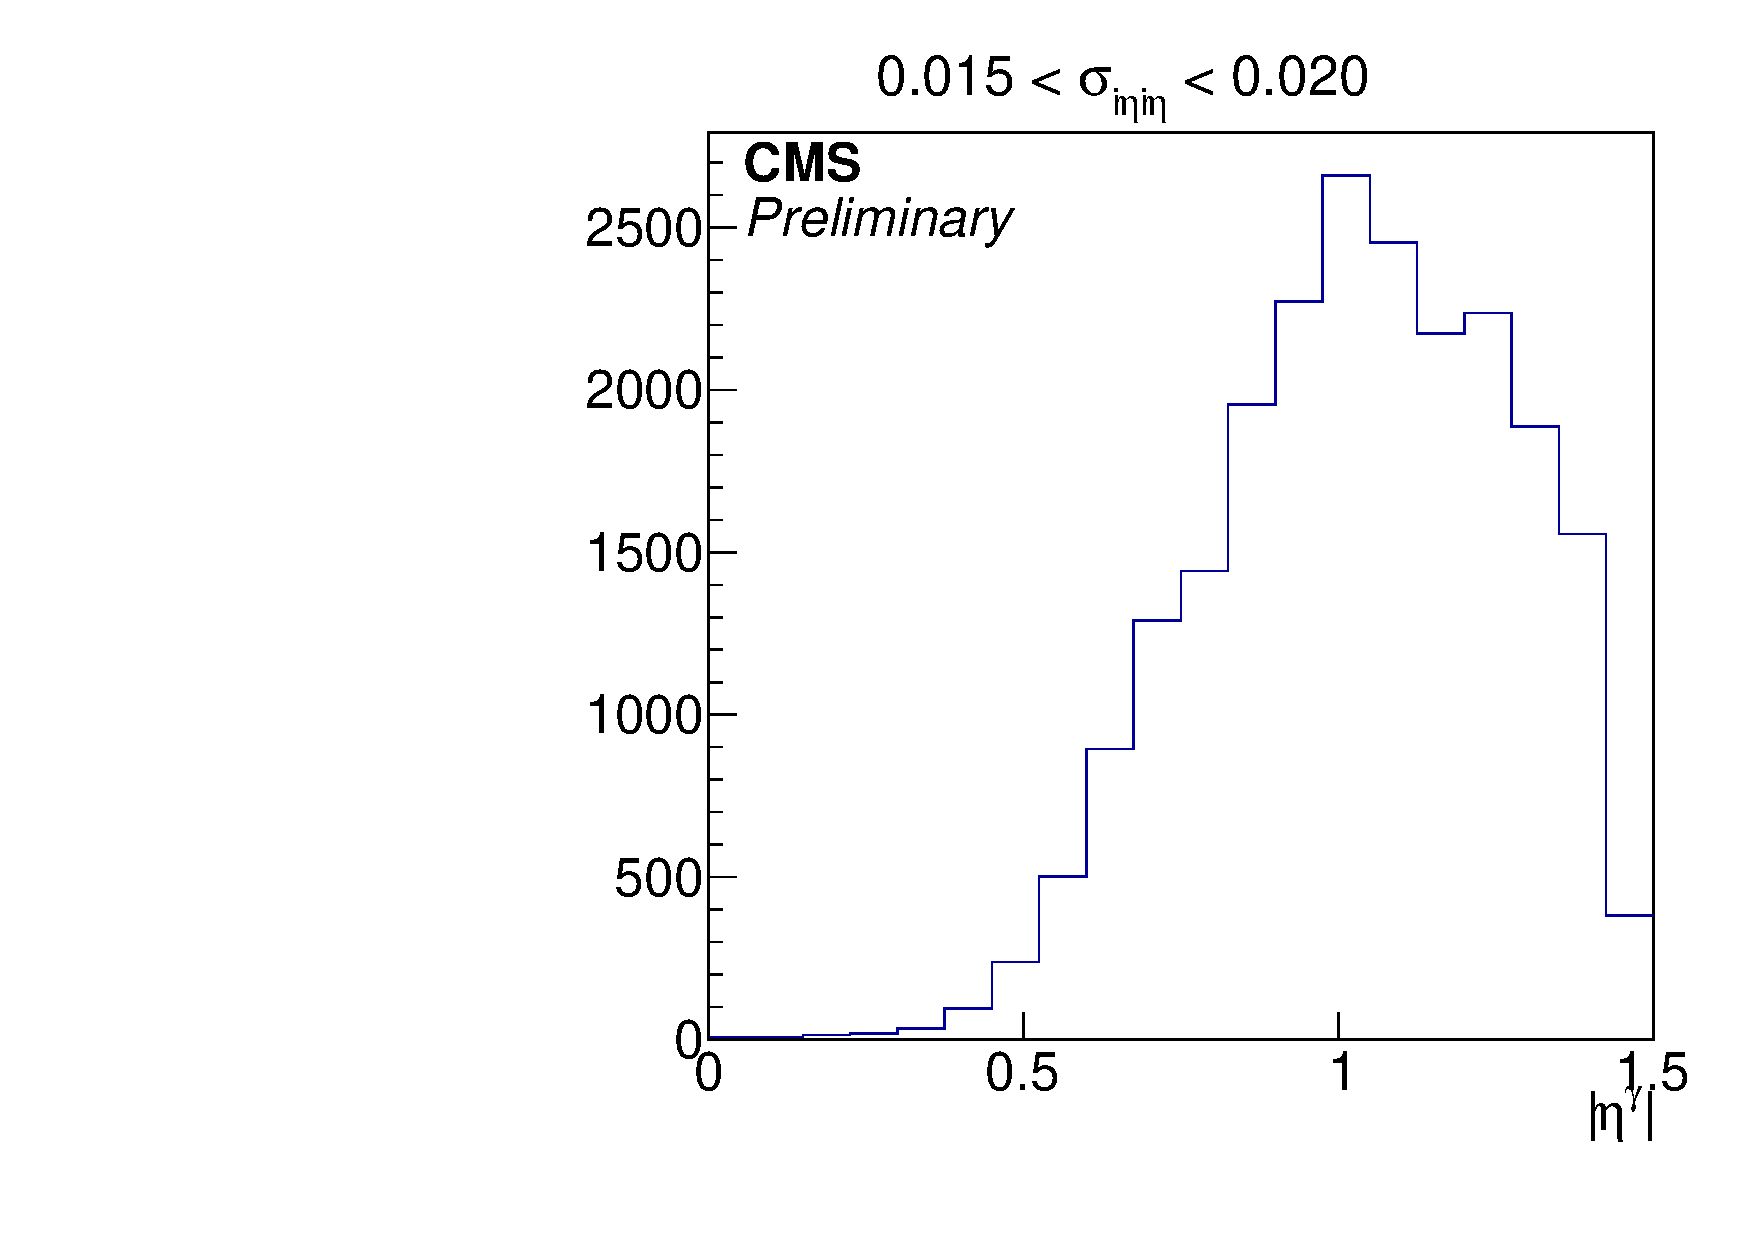
\includegraphics[]{Reconstruction/Figures/halo/halo_shape_etalow.pdf}
    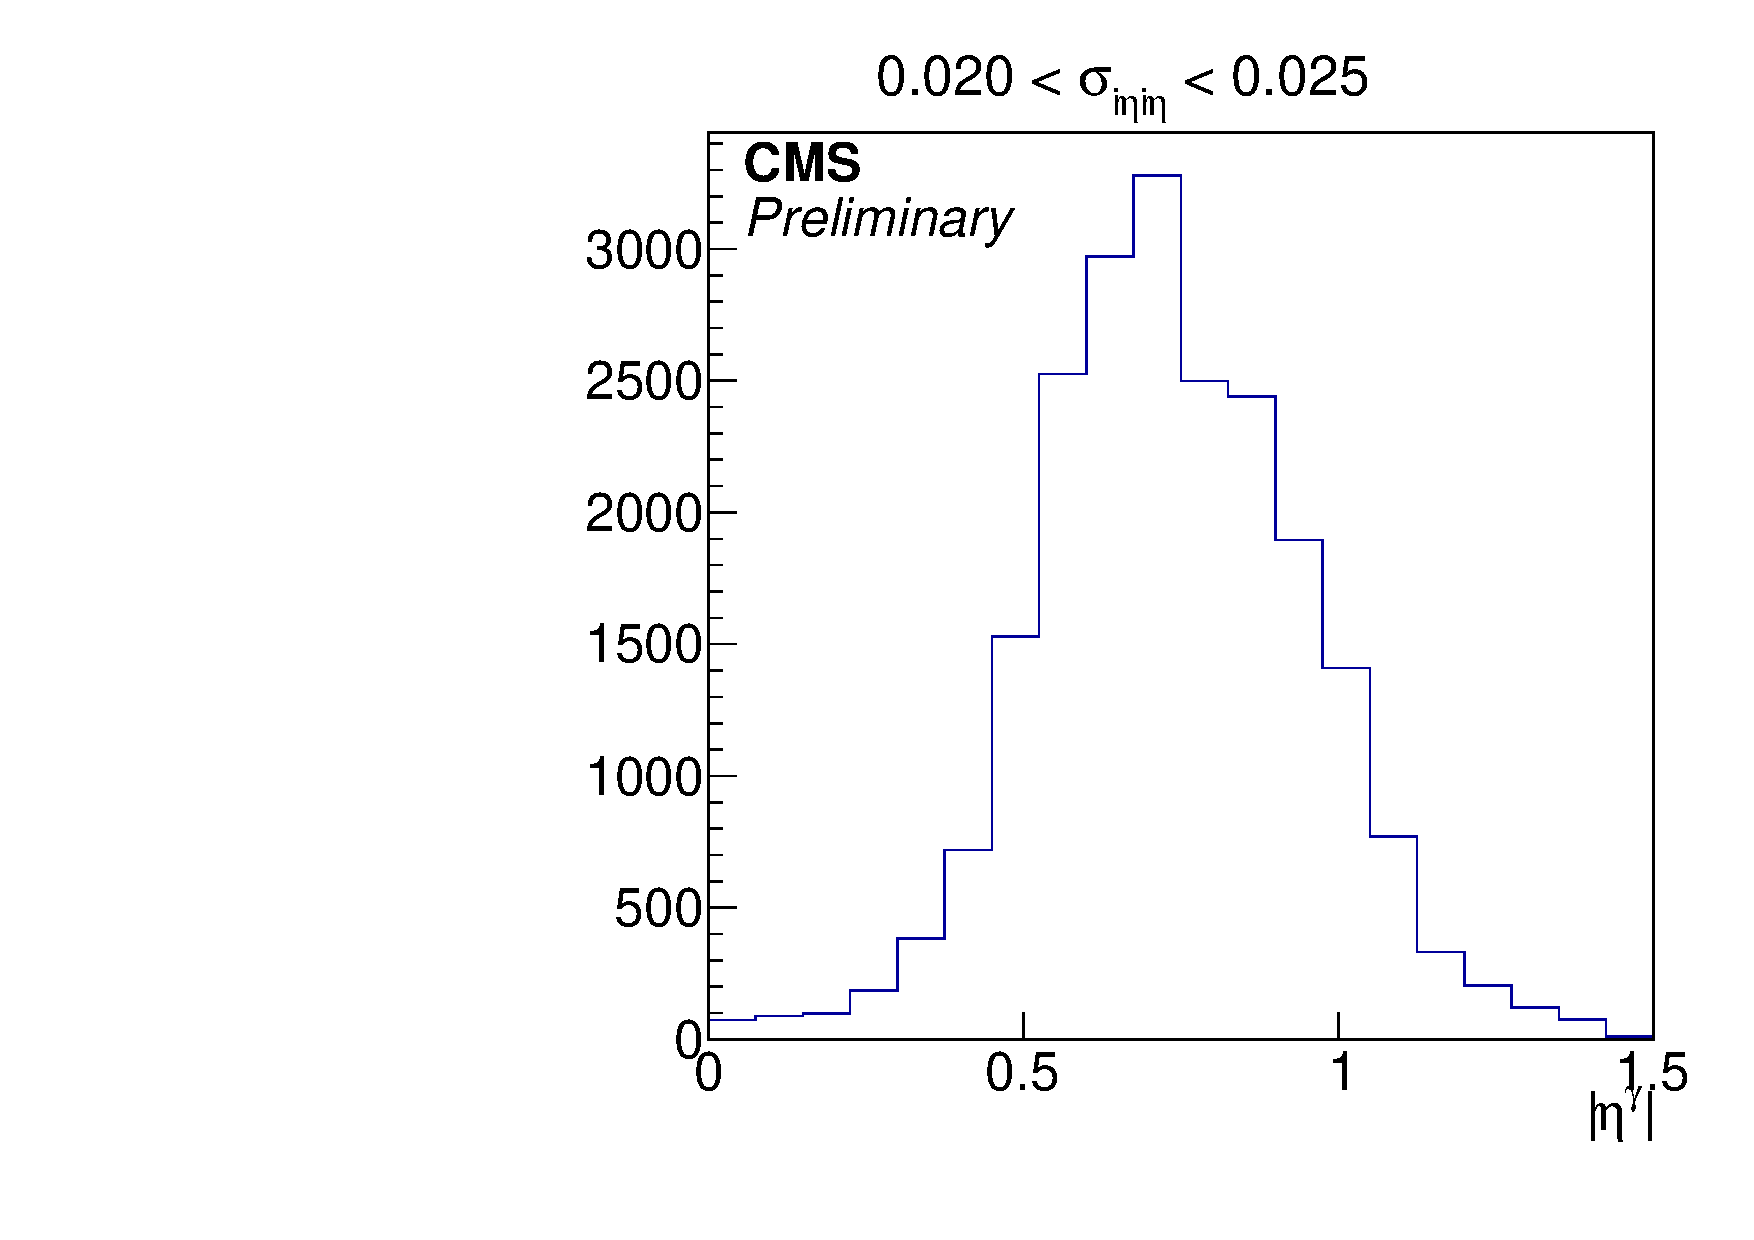
\includegraphics[]{Reconstruction/Figures/halo/halo_shape_etahigh.pdf}
  }
  \caption{
    Left: $\eta$ distribution of the halo-like showers with $|\phi| < \pi/2$ and $|\phi| > \pi/2$.
    Middle and right: shift in the $\eta$ distribution of the halo-like showers with respect to the requirement on \sieie.
    \PH{Please put selection. Label as data. I also don't see the
      point of the two right plots. will read on}
  }
  \label{fig:halo_eta}
\end{figure}

For the distribution of Fig.~\ref{fig:halophi} to be a valid template for halo showers, it must be first confirmed that its shape is invariant under photon selection requirements. 
However, further study of the \phig\ distribution of the halo showers indicates that the relative strength of the two prominent peaks in the distribution may change under the \sieie\ selection requirement.  
To explain this phenomenon, one needs to look at the the \etag\
distribution of the shower populations near $\phig \sim 0$ and $\phig
\sim \pi$, shown in the top portion of
Figure~\ref{fig:halo_eta}. \PH{Please add a sentence explaining the
  effect now I understand why its in the plot. One needs to look make
  me the reader draw the conclusion thats not a good idea here} 
Meanwhile, halo showers tend to have narrower shape in the $\eta$ direction when occurring at high $\eta$, due to the projective geometry of the ECAL crystals, visible in the bottom portion of Figure~\ref{fig:halo_eta} bottom). 
Combining the two observations, the conclusion is that the stringent requirement on the narrowness of the shower in the photon selection will preferentially reduce the $\phi \sim 0$ population.

\begin{figure}[htbp]
  \centering
  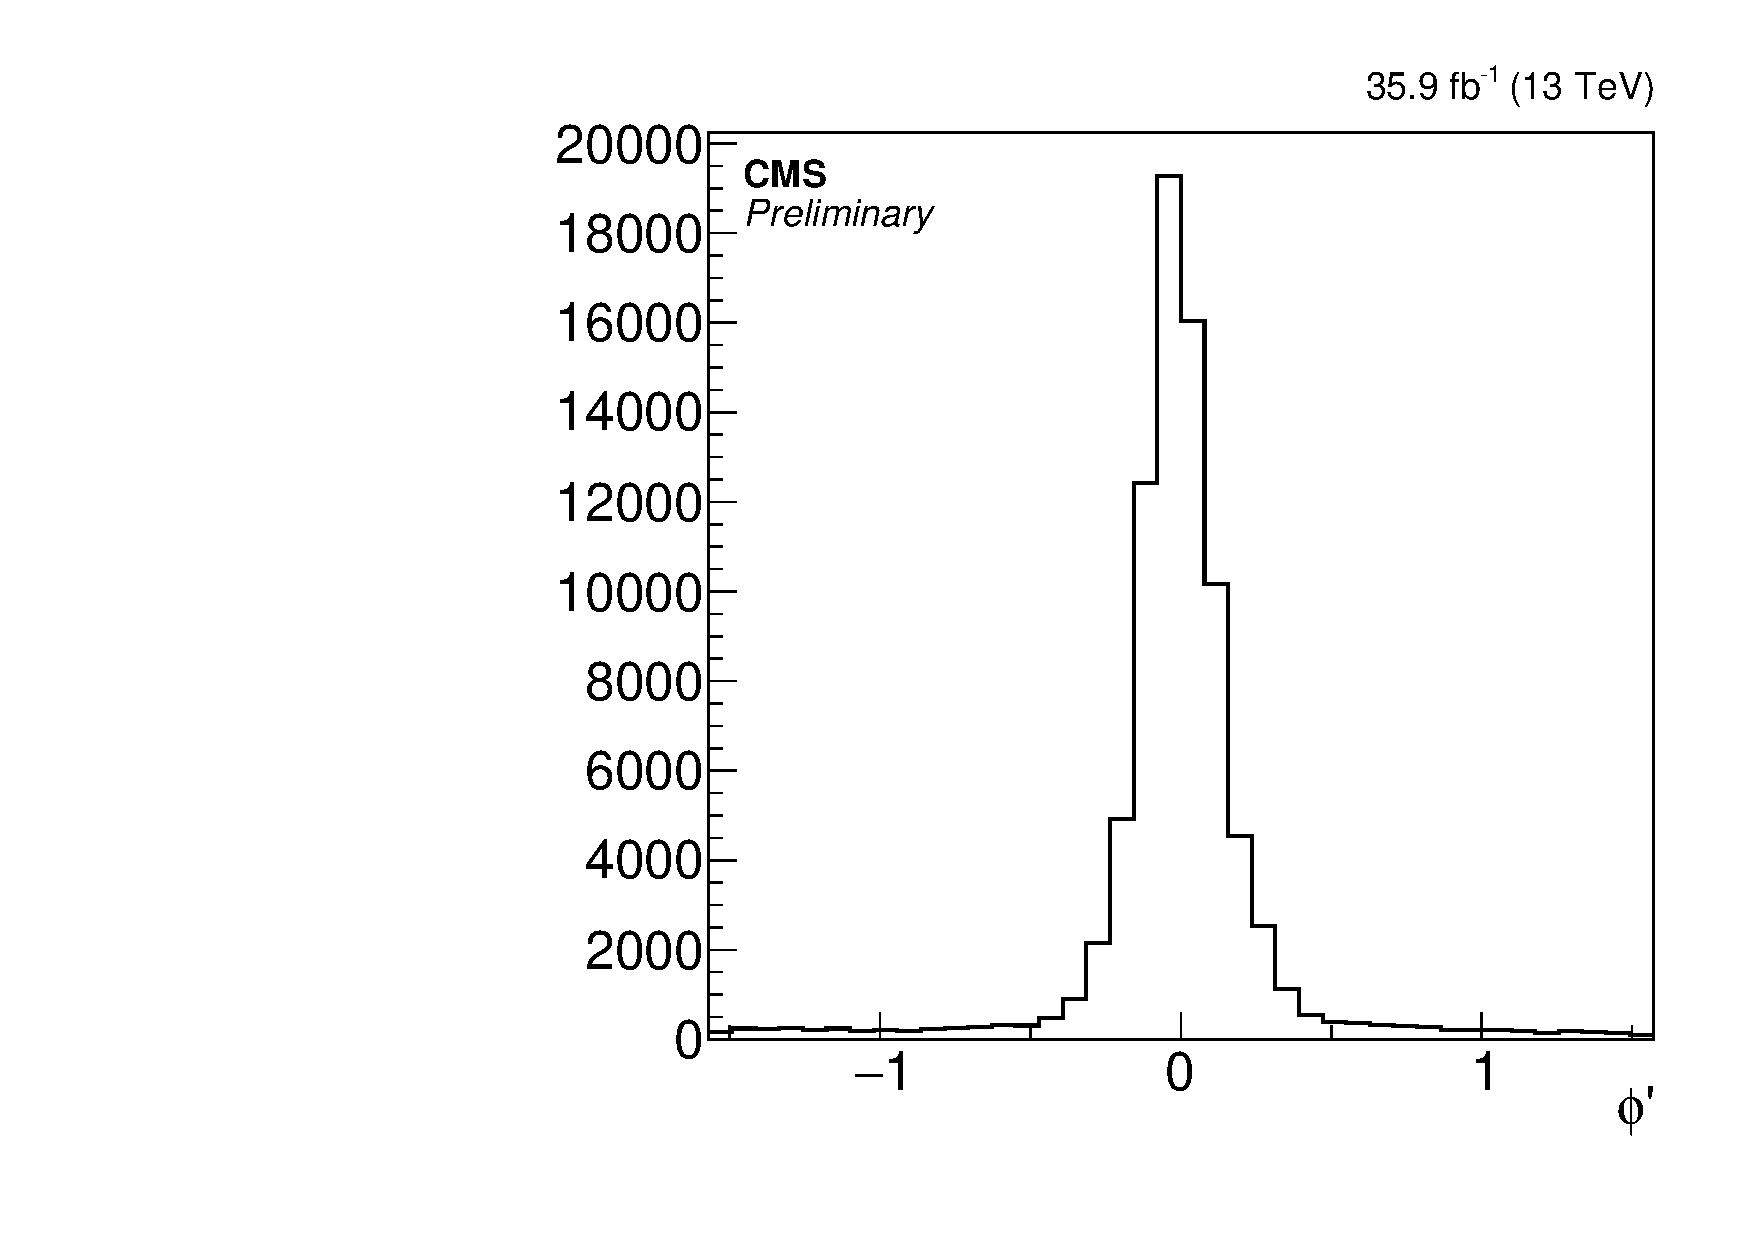
\includegraphics[width=0.35\textwidth]{Reconstruction/Figures/halo/haloPhiFolded.pdf}
  \caption{
    Folded $\phi'$ distribution of the halo sample.
  }
  \label{fig:halo_template}
\end{figure}

Nevertheless, the invariance under photon selection is recovered by folding the \phig\ distribution such that the two peaks of the halo showers coincide.
To match the positions of the peaks in the halo template, the distribution is shifted by 0.005 and then folded along 0. 
The new angular variable $\phi'$
\begin{equation}
  \phi' := \left|\left[\left[\phig + 0.005\right]_{-\pi}^{\pi} - \frac{\pi}{2}\right]_{-\pi}^{\pi}\right| - \frac{\pi}{2},
  \label{eqn:phi}
\end{equation}
where $[\cdot]_{\pi}^{\pi}$ signifies casting the content into range $[-\pi,\pi]$,
exhibits a unimodal distribution for the halo template, as shown in Fig.~\ref{fig:halo_template}.

\begin{figure}[htbp]
  \centering
  \resizebox{\textwidth}{!}{
    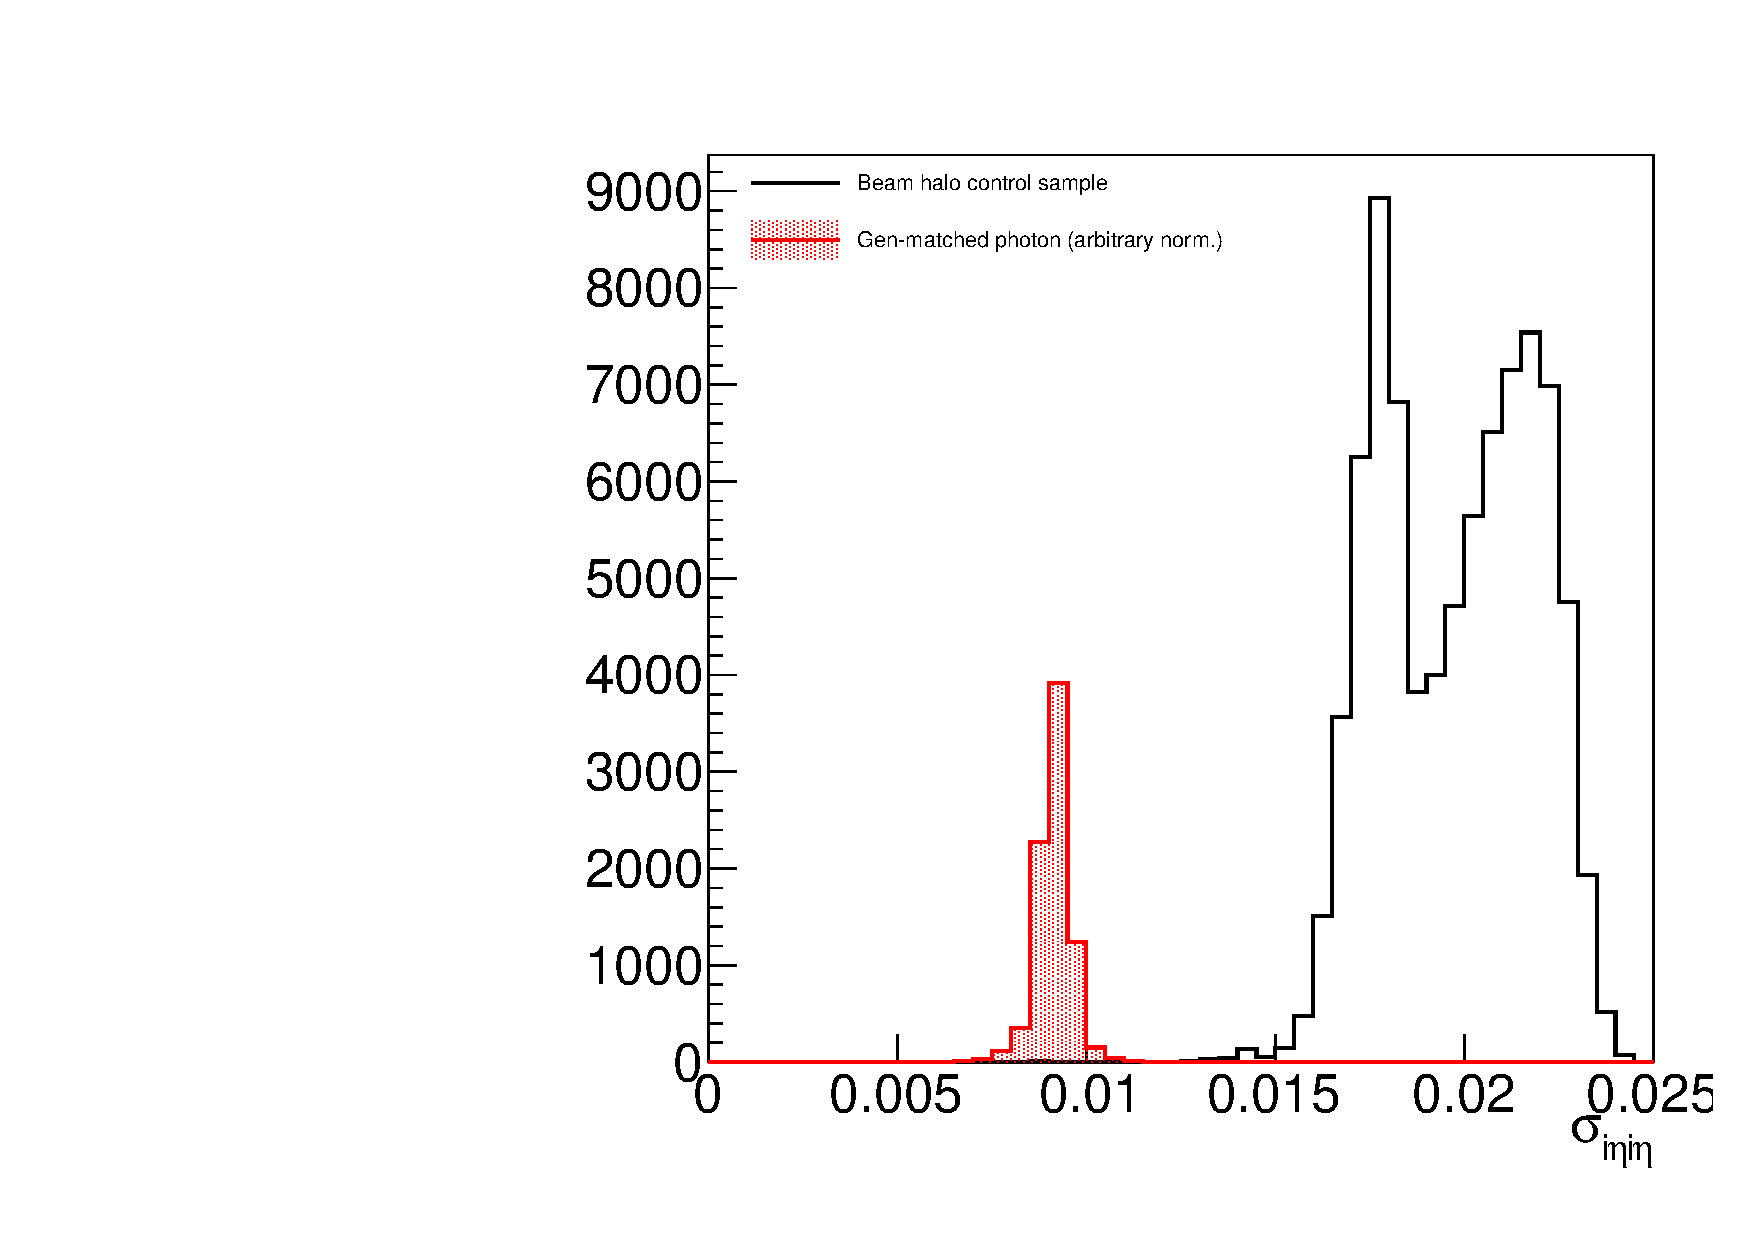
\includegraphics[]{Reconstruction/Figures/halo/halo_sieie.pdf}
    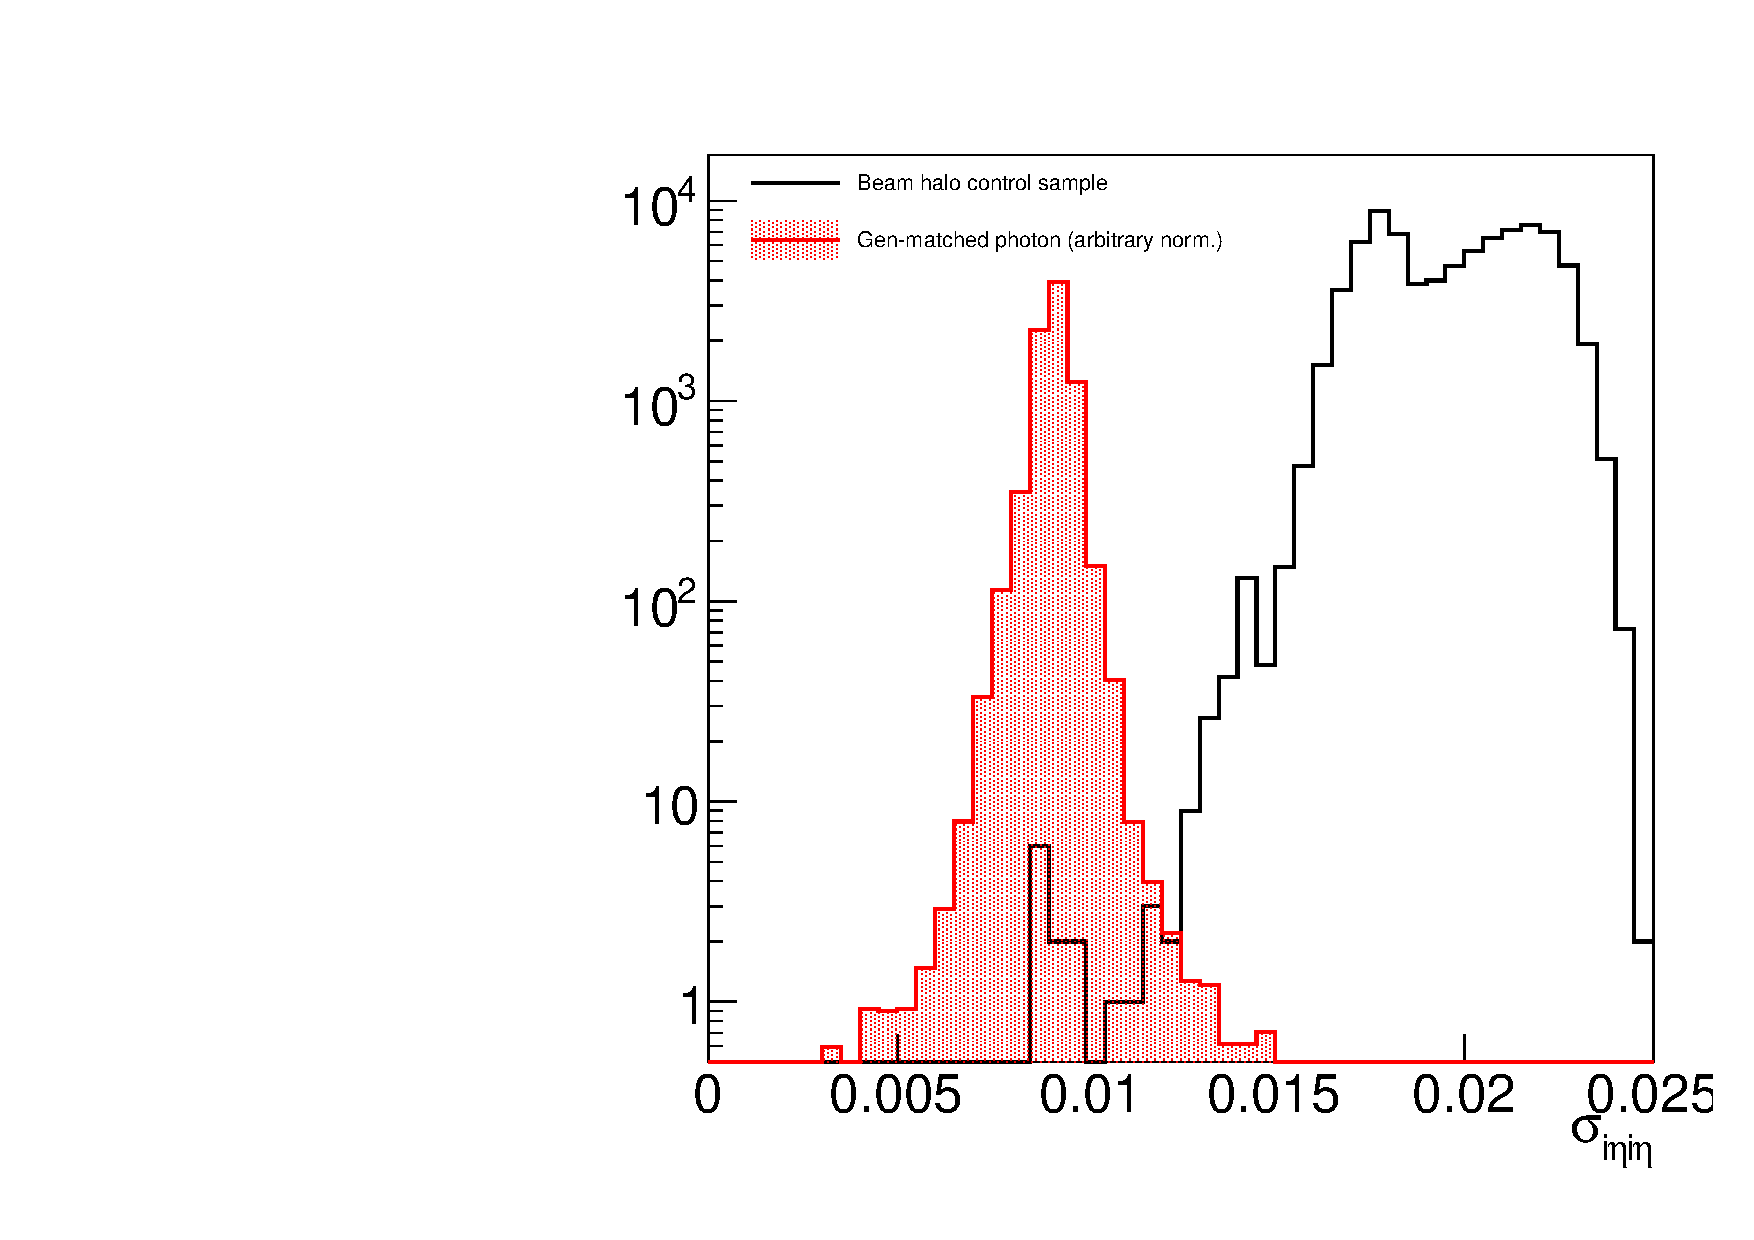
\includegraphics[]{Reconstruction/Figures/halo/halo_sieie_log.pdf}
  }
  \caption{
    The \sieie distribution of the beam halo control sample and a reference distribution from truth-matched MC photons. 
    Left: linear scale, Right: log scale. 
    There is a small peak at $\sieie \sim 0.01$ in the beam halo control sample, which is not visible in linear-scale.
  }
  \label{fig:halo_sieie}
\end{figure}

The contribution of real photons into the halo control sample is negligible.
This is confirmed from the \sieie\ distribution of the halo control sample and the correlation between \sieie\ and \emip\ in a MC true-photon sample.
The \sieie\ distribution of the halo control sample features a small peak at $\sieie \sim 0.01$, which can be attributed to contributions from true photons, as the photon \sieie distribution overlaid in Figure~\ref{fig:halo_sieie} suggests. 
However, the contribution of true photons diminishes rapidly with increasing \sieie. 
Additionally, Figure~\ref{fig:sieie_mip_corr} illustrates that the shape of the true-photon \sieie does not change significantly with respect to \emip. 
From these two observations, we can see that there are is only a negligible number of true photons in the halo control sample.

\begin{figure}[htbp]
  \centering
  \resizebox{\textwidth}{!}{
    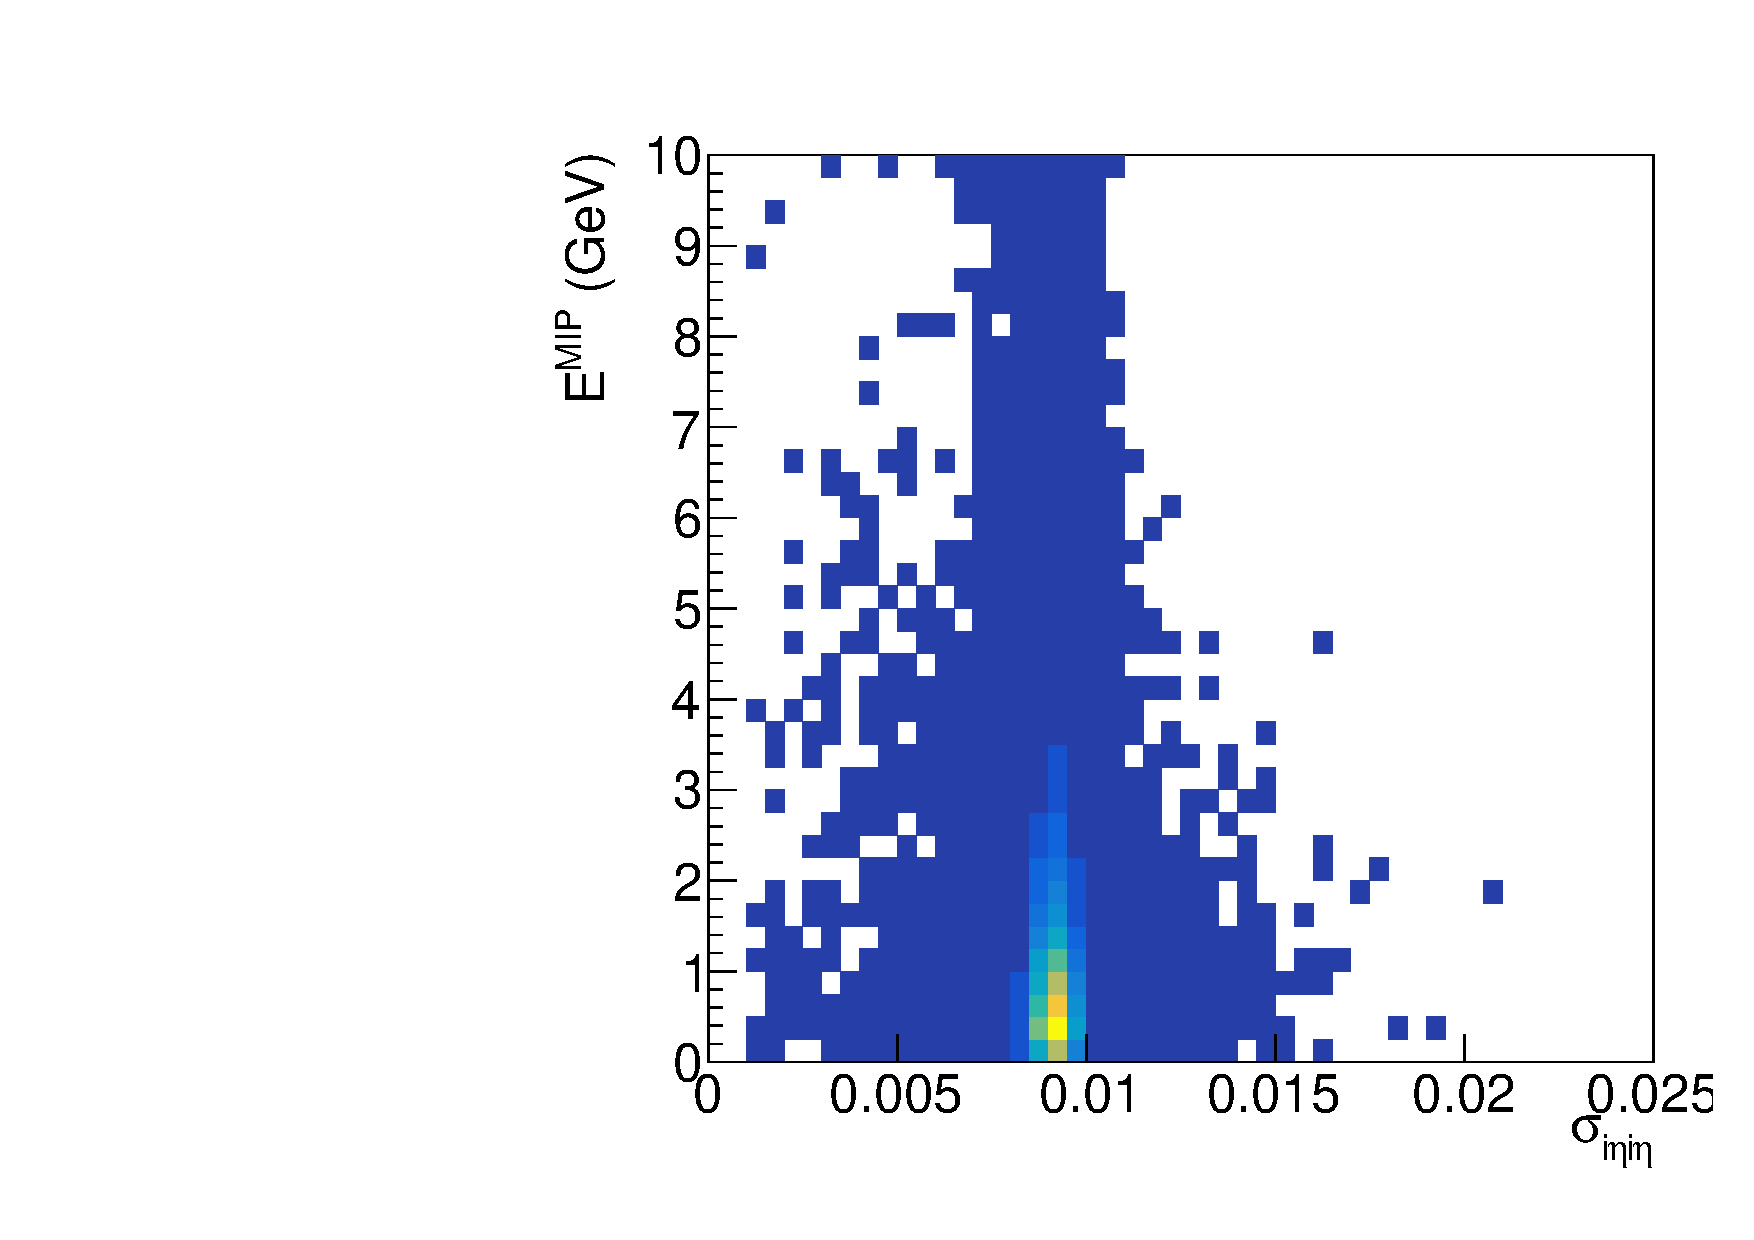
\includegraphics[]{Reconstruction/Figures/halo/sieie_mip_corr.pdf}
    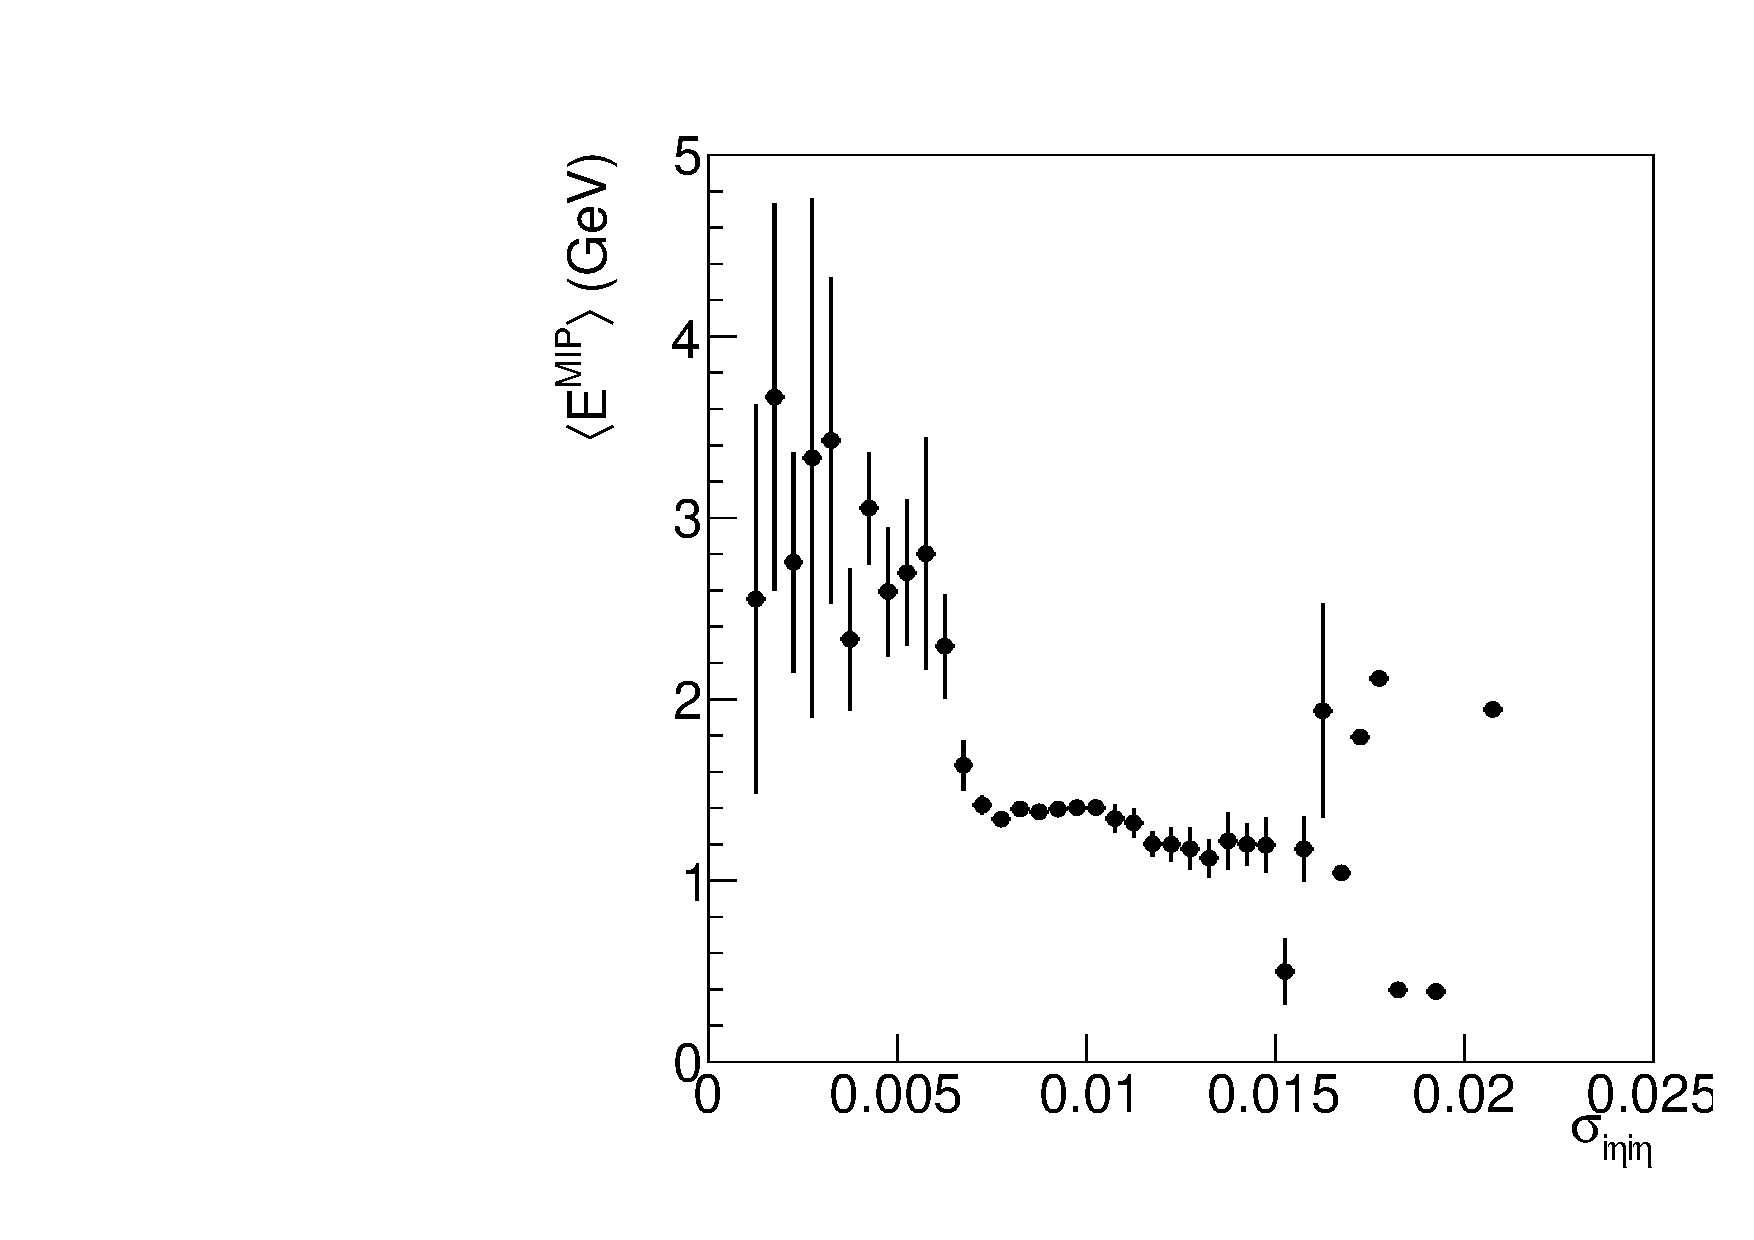
\includegraphics[]{Reconstruction/Figures/halo/sieie_mip_prof.pdf}
  }
  \caption{
    Correlation between \sieie and \emip\ in truth-matched MC photons. 
    Left: \emip-\sieie distribution.
    Right: average \emip\ in bins of \sieie.
  }
  \label{fig:sieie_mip_corr}
\end{figure}
\PH{Not sure what the point of the right plot is}

While the peaking behavior is a robust feature of the halo showers, their rate is not easily predictable. 
Therefore,  a two-template fit to the $\phi'$ distribution of the photons in the candidate sample, where the templates are a uniform distribution (Figure~\ref{fig:halophi} left) and that of the halo shower (Figure~\ref{fig:halo_template}), accurately estimates the amount of beam halo background present in the signal region. 
For this analysis, the splitting of the signal region functions in a similar manner, enabling us to determine the beam halo contribution during the signal extraction procedure.

In the horizontal ($H$) and vertical ($V$) signal regions, collision processes occupy the relative fractions of phase space $C_{H} = 1/\pi$ and $C_{V} = (\pi-1)/\pi$ corresponding to $\abs{\phi'} < 0.5$ and $0.5 < \abs{\phi'} < \pi/2$, respesctively. 
The corresponding fractions for beam halo events are determined by selecting a halo-enriched sample where the halo veto is inverted. 
Thus, a fit of the two signal regions provides an estimate of the overall normalization of the beam halo background, denoted $h$.
 
The \ETg\ dependence of the halo background is encoded in \nhalo[,i], the unit-normalized beam halo prediction in the $i^\mathrm{th}$ bin of the signal region $K \in \{H,V\}$.
Using the notation introduced in Section~\ref{sec:irreducible}, the total estimated background \TK\ in the two signal regions are
\begin{equation}
\begin{aligned}
  \TK[,i] & = C_{K} \left[ \NZg[i] + \NWg[i] + b_{K,i}\right] + h \nhalo[,i]  \\
          & = C_{K} \left( \left[1 + \left(\fZW[i]\right)^{-1}\right) \NZg[i] + b_{K,i}\right] + h \nhalo[,i],
\end{aligned}
\end{equation}
where $b_{K,i}$ is the total contribution to bin $i$ of region $K$ from electron and hadron misidentification, ECAL spikes, and other minor SM background processes.
\PH{The parens are wrong in this formula. Alos, partly because of that
  I can't really follow.}